\documentclass[12pt, oneside, a4paper]{book}

% ----------------------------------------------------------------------------
% Preamble
% ----------------------------------------------------------------------------

% Package to manage page layout
\usepackage[a4paper, top=25.4mm, bottom=25.4mm, right=25.4mm, left=40mm]{geometry}

% Line spacing: single=1 one-and-a-half=1.3 double=1.6
\linespread{1.3}

% Package to manage appendix
\usepackage[toc]{appendix}

% Package to insert empty lines between paragraphs
\usepackage[parfill]{parskip}

% Package to manage headers and footers
\usepackage{fancyhdr}

% define two header-footer styles
% 'normal' for most pages
\fancypagestyle{normal}{
\fancyhf{}
\fancyhead[L]{\slshape \leftmark} %chapter
\fancyhead[R]{\thepage} %footer
\renewcommand{\headrulewidth}{1pt}
}
% 'chapterstyle' for start of chapters (no chapter in header)
\fancypagestyle{chapterstyle}{
    \fancyhf{}
    \fancyhead[R]{\thepage}
    \renewcommand{\headrulewidth}{0pt}% Line at the header invisible
}

% Package to automatically change headerfooter style at start of chapters
\usepackage{etoolbox}
\patchcmd{\chapter}{\thispagestyle{plain}}{\thispagestyle{chapterstyle}}{}{}


% Package to get hyperrlinks
\usepackage{hyperref}

% Mathematics packages
\usepackage{amsmath}
\usepackage{amssymb}
\usepackage{mathtools}

% A package to include graphics files (jpg, png, eps, pdf etc...)
\usepackage{graphicx}
\graphicspath{ {img/} }

% A package that gives more control for bibliographies than the default
\usepackage[backend=biber,
			maxcitenames=2,
			maxbibnames=99,
			doi=false,
			url=false,
			bibstyle=apa,
			firstinits,
			uniquename=init,
			style=authoryear
            ]{biblatex}
\addbibresource{bibliography.bib}


% Package to add features for tables
\usepackage{multirow}
\usepackage{booktabs}
\setlength{\heavyrulewidth}{1.5pt}
\setlength{\abovetopsep}{4pt}

% Package to allow sub-figures
\usepackage{subcaption}


% A package to generate latin. You do not need this: I am just using it to get
% random text.
\usepackage{lipsum}


% ----------------------------------------------------------------------------
% The actual report
% ----------------------------------------------------------------------------

\begin{document}

\newgeometry{a4paper, top=25.4mm, bottom=25.4mm, right=25.4mm, left=25.4mm}
\begin{titlepage}
	\begin{center}
		\vspace*{1cm}
		
\includegraphics[width=3.2cm]{cardiff_logo.jpg} 
		
		\vspace{60pt}
		
		\Huge
		Your Dissertation Title
		
		\vspace{2cm}
		
		\Large
		Your Name
		
		\vspace{2cm}
		\large
		September 2015
		
		\vspace{2cm}
		
		School of Mathematics,\\Cardiff University
		
		\vfill
		
		\normalsize
		A dissertation submitted in partial fulfilment of the\\ requirements for MSc (in
		Operational Research\\ and Applied Statistics) by taught programme.
	
	\end{center}
\end{titlepage}
\restoregeometry

\frontmatter
\pagestyle{chapterstyle} %set header-footer style for front matter
\chapter{Executive Summary}

\lipsum[1-9]
\chapter{Acknowledgements}

\lipsum[1-3]

\tableofcontents
\listoffigures
\listoftables
\chapter{Summary}

\lipsum[1-3]

\mainmatter
\pagestyle{normal} %set header-footer style rest of report


\chapter{Introduction}\label{cha:introduction}

\section{Introduction}

There is this data that is pretty awesome, I'm going to plot it and show it to
you in sections~\ref{sec:the_data} and~\ref{sec:the_distribution_of_the_data}.

\lipsum

\section{The data}\label{sec:the_data}

In Figure~\ref{fig:the_data} we see data that was generated using
(\ref{equ:random_data}):

\begin{equation}
    x \in \{x \in \mathbb{Z}| 1 \leq x \leq 1999\}
\end{equation}

\begin{equation}
    y = 2(1 + \epsilon) x + 5\label{equ:random_data}
\end{equation}

where \(\epsilon\in(-0.5, 0.5)\) is a random number.

\begin{figure}[!hbtp]
    \begin{center}
        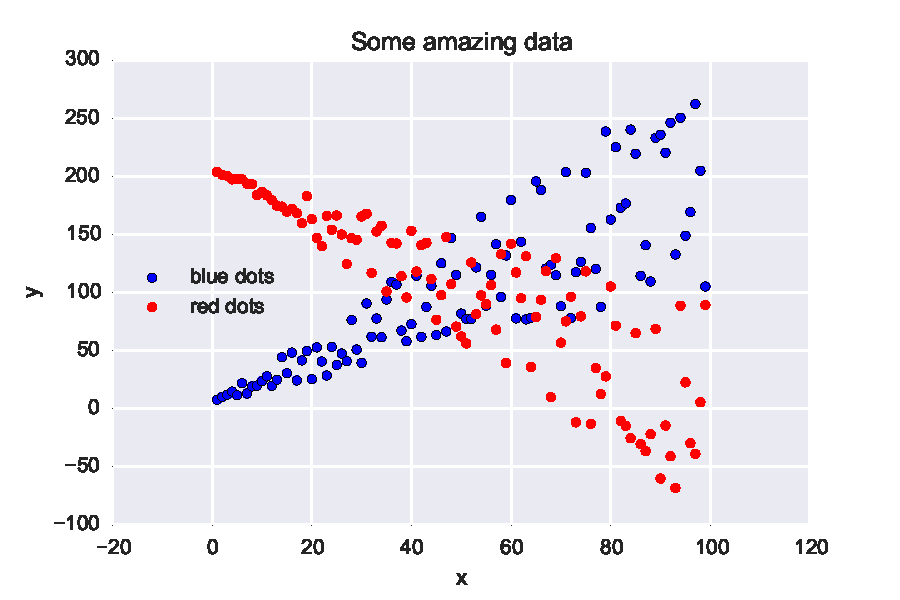
\includegraphics[width=.6\textwidth]{../img/plot1.pdf}
        \caption{The great data}\label{fig:the_data}
    \end{center}
\end{figure}

\section{The distribution of the data}\label{sec:the_distribution_of_the_data}

Figure shows the distribution of the data.

\begin{figure}[!hbtp]
    \begin{center}
        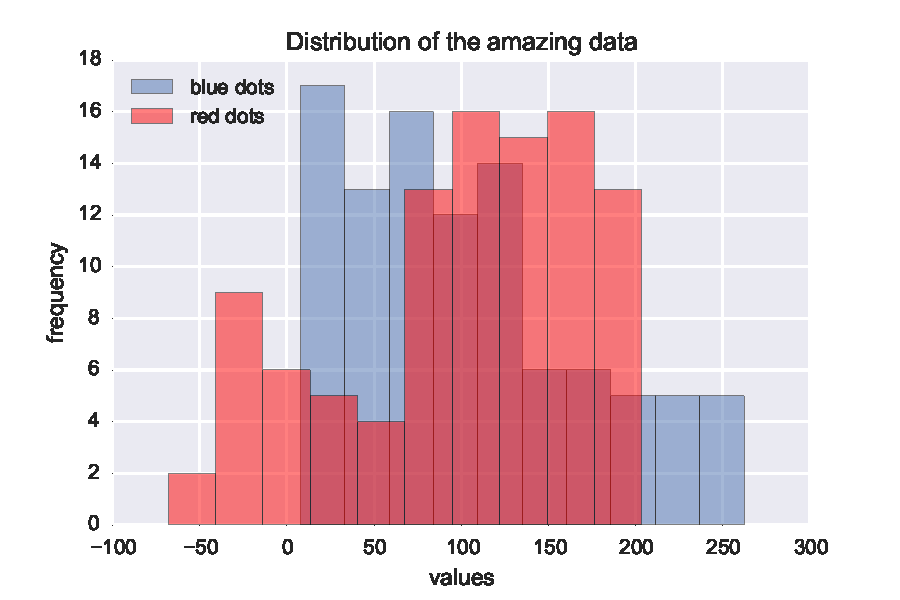
\includegraphics[width=.6\textwidth]{../img/plot2.pdf}
        \caption{The distribution of the great data}\label{fig:the_distribution_of_the_data}
    \end{center}
\end{figure}

\lipsum

\section{Conclusion}\label{sec:conclusion}

This chapter was amazing, here is a reference to a paper~\cite{Gillard2014}.


\chapter{Awesome theorems and stuff}\label{cha:awesome_theorems_and_stuff}

\section{Introduction}

Note that I can refer to other chapters: see Chapter~\ref{cha:introduction} and
even specific equations in each chapter, this is an
equation~(\ref{equ:random_data}).

\lipsum

\chapter{Title of Chapter 3}

\lipsum[1-10]
\chapter{Title of Chapter 3}

\lipsum[1-10]



\addcontentsline{toc}{chapter}{References}
\printbibliography[title=References]

\begin{appendices}
\chapter{First Appendix Title}

\lipsum[1-2]

\chapter{Second Appendix Title}

\lipsum[1-2]
\end{appendices}

\end{document}
